\documentclass[lecture.tex]{subfiles}

\begin{document}

\exercice{Jessy Lefeuve}
%\video{https://youtu.be/blablabla}
\enonce{rdm-0021}{Contraintes}

\begin{figure}[h]
  \centering
  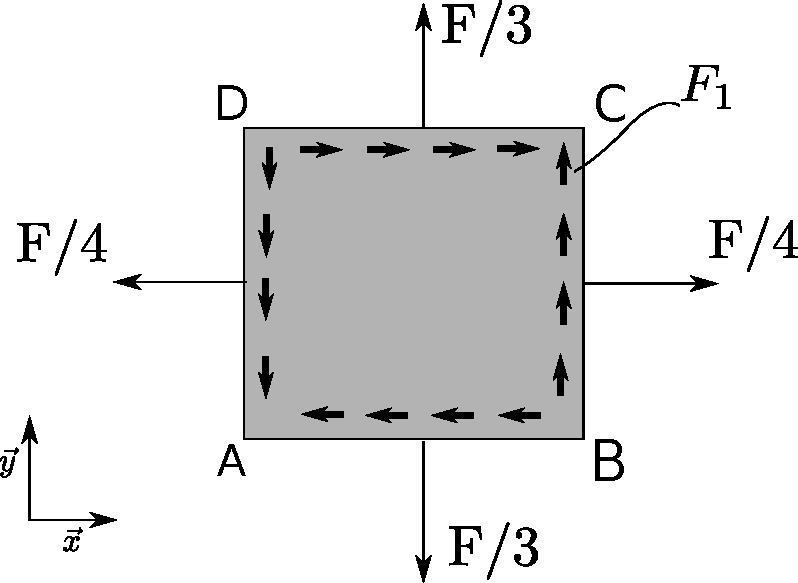
\includegraphics[scale=0.5]{Contrainte_Tole.pdf}
  \caption{Tôle sous contraintes}
  \label{Tole_C}
\end{figure}

Soit une tôle carrée de côté $a$ et d'épaisseur $e$ très faible de telle sorte que les contraintes sont considérées planes. Chaque côté de la tôle est soumis à un effort orienté positivement selon la normale sortante:

\begin{itemize}
  \item[$\bullet$] Sur les côtés AD et BC: de valeur $F/4$
  \item[$\bullet$] Sur les côtés DC et AB: de valeur $F/3$
\end{itemize}

En outre, les côtés AB, BC, CD et AD sont soumis à un effort réparti $F_1$ (Newton) de telle sorte que la tôle reste statique. La figure (fig.\ref{Tole_C}) résume l'ensemble des efforts appliqués sur la structure.

\begin{enumerate}
  \item Trouver les contraintes tangentielle $\sigma_{xy}$.
  \item Trouver les contraintes normales $\sigma_{xx}$ et $\sigma_{yy}$.
  \item Exprimez le tenseur des contraintes en un point M de la tôle $\Sigma_M$.
\end{enumerate}

\finenonce{rdm-0021}
\finexercice

\end{document}
